%*****************************************
\chapter{Implementation}\label{ch:implementation}
%*****************************************

Um die Webanwendung platformübergreifend entwickeln und auf beliebigen Systemen einsetzen zu können würde ASP.NET Core MVC als Development Framework gewählt.

\section{ASP.NET Core MVC}

Die General-Purpose-Development-Platform .NET Core wurde unter Koordination von Microsoft zusammen mit der .NET Community entwickelt und als Open Source-Projekt über GitHub \cite{dotnetcore} verfügbar gemacht. Sie bietet eine platformübergreifende Lösung zur Entwicklung und Ausführung von Anwendungsprogrammen und läuft unter Windows, macOS and Linux. ASP.NET steht für Active Server Pages .NET und ist ein Web Application Framework von Microsoft, mit dem sich dynamische Webseiten, Webanwendungen und Webservices entwickeln lassen. ASP.NET Core MVC baut auf .NET Core auf und vereint die Effektivität und Übersichtlichkeit der Model-View-Controller (MVC) Architektur \cite{freeman2016pro}. Als Entwicklungsumgebung wurde Visual Studio Code, ein kostenloser und quelloffener Texteditor, mit C\# Extension genutzt.

\subsection{Model-View-Controller}

Das Model-View-Controller Design Pattern dient der Trennung der Software in die drei Komponenten Datenmodell (engl. model), Präsentation (engl. view) und Programmsteuerung (engl. controller). Beim MVC-Pattern werden eingehende Anfragen durch Controller behandelt. In ASP.NET Core MVC sind Controller C\#-Klassen die gewöhnlich von der integrierten MVC-Controller Basisklasse \code{Microsoft.AspNetCore.Mvc.Controller} erben. Jede \code{public}-Methode eines Controllers wird auch Action Method genannt. Man kann sie aus dem Web über eine URL aufrufen und so eine Aktion ausführen. In einer Web Application geht es darum dynamischen Output zu konstruieren und darzustellen. In MVC ist der Controller dafür zuständig basierend auf dem Model Daten zu konstruieren und diese an den View weiterzugeben, welcher wiederum das HTML rendert. Dies ist in Abbildung \ref{fig:mvc} dargestellt.

\begin{figure}
\centering
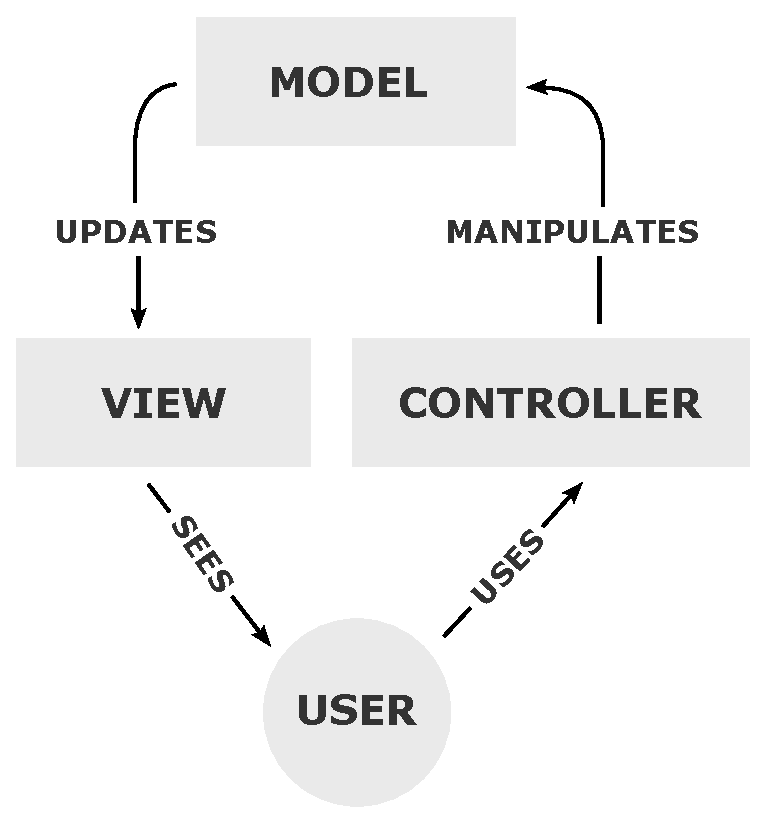
\includegraphics[width=6cm]{Figures/mvc}
\caption{Model-View-Controller}
\label{fig:mvc}
\end{figure}


\subsection{Routes}

ASP.NET Core MVC Applications nutzen das ASP.NET routing system. Diese entschiedet welche URLs auf welchen Controller und welche Actions abgebildet werden. Eine Route ist eine Regel die darüber entscheidet wie eine Anfrage behandelt wird. Als Standardregeln für ein neues MVC Projekt sind werden beispielsweise die folgenden URLs auf die Index action des code{HomeControllers}s weitergeleitet.

\begin{itemize}

	\item /
	\item /Home
	\item /Home/Index

\end{itemize}

\noindent
Nach Konvention hat die Application einen \code{HomeController} welcher den Einstiegspunkt in die MVC Application bidlet.

\subsection{Razor view engine}
